
 \section{Startup}
\label{sec:startup}

The term became popular during the dotcom bubble, when a great number of companies were founded to do business on the Internet. Steve Blank lists some principles of a startup in his blog post "What’s A Startup? First Principles.". Blank defines a startup as "an organization formed to search for a repeatable and scalable business model". The first goal for a business model can be revenue, profits, users or click-throughs. The business model must be quickly and constantly tested and iterated by using Agile Development. Blank also tells that the business model of most startups is changed multiple times.~\cite{blank2010startup}

 \subsection{Lean Startup}
 
Lean Startup is a movement pioneered by Eric Ries, which brings the principles of lean manufacturing to the context of entrepreneurship. Like the lean manufacturing is measuring progress also the lean startup measures its progress for discovering and eliminating the sources of waste. Lean manufacturing measures the progress by the production of high-quality goods, whereas in lean startup, the unit of progress is something Ries calls validated learning.~\cite{ries2011lean}

Ries' definition of a startup is "a human institution designed to create a new product or service under conditions of extreme uncertainty". This definition omits the size of the institution and thus implies that a startup can be ranging from an individual or a small group of people to a team or division inside a large company. The most important aspect of the definition is the extreme uncertainty, which needs constant measurement and steering of the process.

There are five principles in Lean Startup~\cite{ries2011lean}:

 % 5 principles

\textbf{1. Entrepreneurs are everywhere.} Entrepreneurship involves everyone working inside a human institution in where new products and services are created under uncertain conditions. This means that Lean Startup approach can be applied in any size company from a single person working in a garage to even a large enterprise, leaving no industry out.

\textbf{2. Entrepreneurship is management.} Treating a startup as just a product is not a valid approach. A startup is an institution having constant uncertainty present, so it requires new kind of management.

\textbf{3. Validated learning.} Startups exist primarily for learning how to build a sustainable business. This learning can be validated using frequent experiments for testing the vision.

\textbf{4. Build-Measure-Learn.} The main function of a startup is to turn ideas into products, measure the customer response and then learn whether to pivot or persevere. All successful startup processes should be aimed to accelerate the feedback loop shown in Figure~\ref{fig:feedback-loop}

\textbf{5. Innovation accounting.} Improving the outcome of entrepreneurs and holding innovators accountable means focusing on measuring the progress, setting milestones and prioritizing work. This requires new kind of accounting designed for startups.

\begin{figure}[t]
\begin{center}
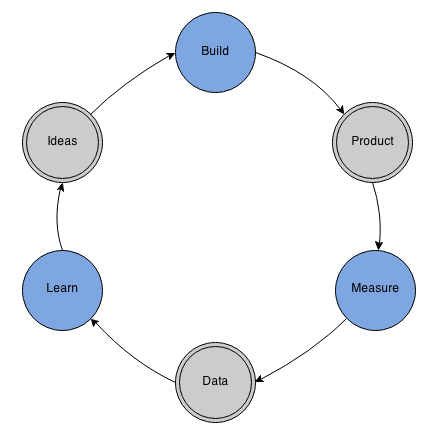
\includegraphics[width=0.5\textwidth]{image/feedback-loop.png}
\end{center}
\caption{Build-Measure-Learn feedback loop}
\label{fig:feedback-loop}
\end{figure}

% -Datan keruu \& oppiminen



 \subsection{Life Cycle in Lean Startup}

 
 The life cycle in a Lean startup software development doesn't match to the traditional life cycle of a software product. In building a successive product for a software startup, there are usually multiple short iterations surveying the context in which the product will be used. Building a software startup can be started without knowing what the customers want or even who the customers are, so the life cycle of the product has to be built from multiple consecutive version with significant and rapid changes for conforming to the customers demands.~\cite{ries2011lean}

The basic repeating process of development in Lean Startup begins from an idea. This idea contains usually several hypotheses about the customer behavior or the context of usage. Some of these are called leap of faith assumptions, which are the riskiest hypotheses of the plan. Using these hypotheses for validated learning, allows avoiding much of the waste usually present in startups. To utilize the validated learning as a scientific method, there needs to be a selected group of hypotheses to test. The leap of faith assumptions should be the first ones to be tested, because they are the foundation on which the business is to be built. Testing the first hypotheses can be sometimes done with virtually nothing built. This has been done for example by the founder of the online shoe store Zappos, who sold the first pairs of shoes without having any inventory of his own but only some pictures of shoes taken in local shops.~\cite{ries2011lean}

When the first hypotheses have been proved true, hopefully with only a small effort, the Build phase can be initiated and the first minimum viable product (MVP) can be built. This product is a version which enables a full turn of the Build-Measure-Learn loop with minimum effort. This MVP is usually missing most of the features that will be proven essential later. The purpose of this version is that it must be able to measure its impact. The target audience of this product is not the development team or some business heads, but the potential customers, so it can evaluate the reactions of the market.~\cite{ries2011lean}

After the MVP is released, the startup enters the Measure phase. In this phase, the most important topic to get answer for is whether the product development efforts are leading to real progress. In other words: is the product something someone wants. If building something that nobody wants, there is no sense in using time and money on the development. Ries suggests doing the measuring with a method called innovation accounting. It is a quantitative approach for testing if the tuning is successful. It allows creating learning milestones, which are useful for the entrepreneurs for evaluating their progress accurately.~\cite{ries2011lean}

Once the entrepreneurs have learned from the measurements done, it is time for the most important step in the cycle. In this step, the entrepreneurs must assess the success of the hypotheses and based on these assessments, they must decide whether to pivot the original strategy or persevere. If any of the hypotheses proved to be false, it is time for pivot: to make a major change to a new strategic hypothesis. One of the most important objective of the Lean Startup is to allow the recognition of the time to pivot soon, wasting less time and money.~\cite{ries2011lean}

Even though this cycle is called Build-Measure-Learn according to the order of execution, the planning of the cycle is done backwards. The first thing to plan is what is needed to learn. Then using innovation accounting, the things needed to measure are figured out. The last thing is to design the product able to run the experiment returning the measurements.~\cite{ries2011lean}

 Eric Ries reveals multiple success stories using Lean Startup, in where there are many similarities. One of the success stories is about a collaboration portal for voters. The first released version of the portal was achieved with 1200\$ and three months of work. With that version, some of the assumptions could be tested in the real operating environment and the product could be developed further. After the partial success of the first version, there were five other version of the portal and the business model developed. After each of the launches, the leaps of faith were tested and the necessary changes were made for steering the product to the right direction. After 16 months of development the product had reached a sufficient state for a sustainable business. During these months, there had been several pivots and changes, which cannot be seen as a traditional product life cycle.~\cite{ries2011lean}:



% Tässä scopessa ei perinteisessä mielessä life cycleä
% Iteratiivista kehitystä, MVP, continuous deploymentia ja pivoteja
% http://blogs-images.forbes.com/martinzwilling/files/2013/02/valley-of-death.jpg
% Votizen p.150
%	-5 MVP:tä 

% \begin{itemize}

% \item Startup financing cycle (Valley of Death)
% \item Iteratiivinen kehitys
% \item Lyhyet sprintit
 
% \end{itemize}
 
% \subsection{Product scope}
 
%PMBOK p. 51 Project scope management
%	-Product scope
%	-Project scope


% \begin{itemize}
 
% \item Analytics
% \item Ominaisuuksien priorisointi (esim. käytön mukaan)
% \item Scope
% \item MVP
% \item Valitaan oikeat feature
% \item Validoinnit: I Know I When I See It
% \item Leanista jotain tännekin
 
% \end{itemize}
 